\chapter{Securing Applications}
\label{ch:unmodified_app}
TrustZone was first announced in the year 2004 ~\cite{trustzone}, and has since been used for a diverse
range of applications as can be seen in section \ref{sec:related}. Some of these applications target new use-cases that can benefit from the guarantees a TEE provides, while in other cases, pre-existing applications are re-structured and re-factored to make use of a TEE. How these projects structure their secure applications roughly falls into five distinct categories which differ based on the information being protected and the threat model around which the application has been designed: 

%%%%%%%%%%%%%%%%%%%%%%%%%%%%%%%%%%%%%%%%%%%%%%%%%%%%%%%%
\begin{figure}[t]
    \centering
    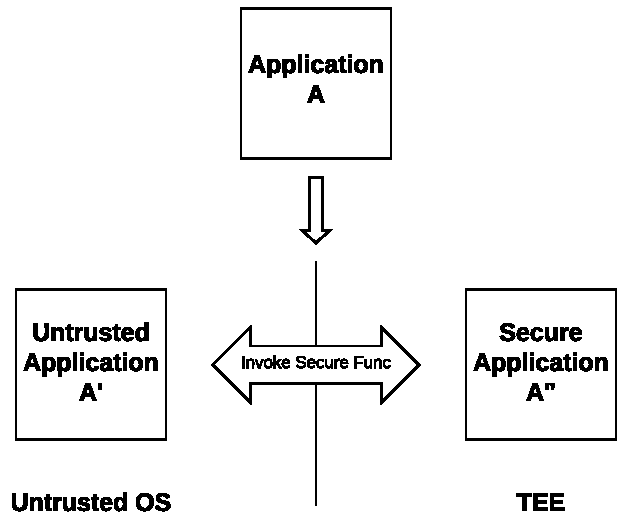
\includegraphics{fig/split_app.pdf}
    \caption{An application can be split into two parts - one that resides in the untrusted operating system and has the interfaces to secure functionality that resides in the trusted environment.}
    \label{fig:split_app}
\end{figure}
%%%%%%%%%%%%%%%%%%%%%%%%%%%%%%%%%%%%%%%%%%%%%%%%%%%%%%%%



\begin{enumerate}
    \item \textbf{Manually Split the Application into Trusted and Untrusted
    Parts:} This is the most commonly used methodology designing applications
    with the view to use a TEE to safeguard some aspect of the program state 
    \cite{TLR,Proxos,SchrodinText,liu2014veriui}. 
    
    The basic idea is that there is some easily identifiable functionality that
    can be plucked out of the monolithic application and can be offloaded to the
    TEE. The rest of the application that remains on the untrusted OS only has interfaces to the secure functions in the TEE. This is shown in Figure
    \ref{fig:split_app}. The TEE in this scenario could either be a trusted operating system that is hosted as a virtual machine or it could be a
    more conventional hardware-based TEE like Intel's SGX or ARM's TrustZone. 

    This application splitting paradigm is promising in scenarios where the critical functionality that needs protection is small, well defined, and can be extracted out into a TEE-resident service. Prime examples of this are biometric verification, cryptographic functions, payment processing, and verifying the user's action and intent. An implicit assumption with this strategy is that the partitioning of the application is a deliberate decision that is made at the time of designing the application and therefore can not be used for an unmodified application. 
    
    \item \textbf{Compiler Supported Application Sequestering}: There has been work in securing application using compiler wizardry. VirtualGhost
    \cite{criswell2014virtual} defines a compiler-based instrumentation of the
    kernel and the application to protect the applications data confidentiality
    and integrity. The OS is compiled to a virtual instruction set which is
    handled by the Virtual Ghost VM as shown in Figure \ref{fig:compiler_split}.
    This \say{virtual machine} is used to limit the accesses the kernel has into the state of the application. This is an interesting work that provides strong guarantees about the application's integrity and data confidentiality without using a hardware-based TEE. 
    
    There has been work in automatically identifying which parts of the application need to be protected and splitting the application using the TEE API \cite{rubinov2016automated, lind2017glamdring}. This approach involves using static analysis and dataflow analysis along with optional annotations in the program to automatically identify the partitioning scheme, and then refactoring the application into two parts that are bridged using the TEE API. Programming language theory can be used to demonstrate equivalence between the split halves and the original application. 

    These approaches might be an efficient way to retroactively make an
    unmodified application ready for a TEE.
    %%%%%%%%%%%%%%%%%%%%%%%%%%%%%%%%%%%%%%%%%%%%%%%%%%%%%%%%
    \begin{figure}[t]
        \centering
        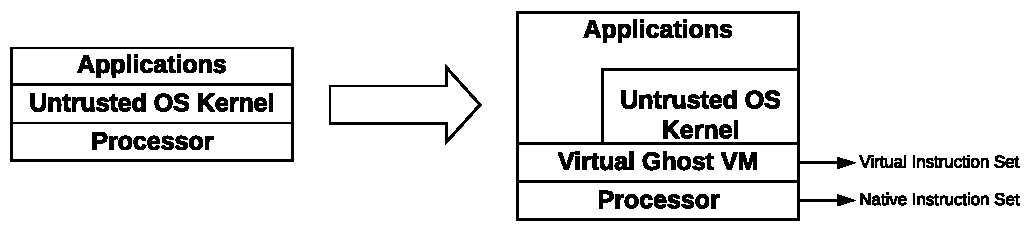
\includegraphics[width=\linewidth]{fig/compiler_split.pdf}
        \caption{Virtual Ghost uses LLVM to create an intermediate layer  the OS and the processor to protect the application from the unfettered access otherwise enjoyed  by a kernel}
        \label{fig:compiler_split}
    \end{figure}
    %%%%%%%%%%%%%%%%%%%%%%%%%%%%%%%%%%%%%%%%%%%%%%%%%%%%%%%%

    \item \textbf{Complete Isolation of the Application Inside the Secure World}
    This approach is, in theory, the path of least resistance to use a TEE. There have been some projects that try to contain an entire application in the TEE - Graphene ~\cite{TsaiGraphene2014,tsai2017graphene} and TrustShadow ~\cite{trustshadow}, for example. These systems rely on the TEE to make available all services that the application might require - most importantly the I/O and peripheral access and the system call interface. This approach, while promising, is fraught with its own set of problems. TEE's are a restrictive execution environments - Intel SGX, for example, does not provide access to a system call interface. No application running in SGX is allowed to make a system call. Similarly, in TrustZone and specifically OP-TEE, because the TEE OS is minimalist, it is difficult to support a full-fledged application. It is for this reason that a significant part of the effort is spent in trying to create port functionality in 
    
    \item \textbf{System Call Interception }
    If the complete isolation of an application is not possible, and it is
    necessary to maintain some part of the application in the untrusted OS, the
    most enticing option available to the security engineer is to use system
    call interception in the normal world OS and handle the \say{sensitive}
    accesses to data and the network in the TEE. This approach can go awry if there is not a strict control on the number and type of system calls that are handled in the TEE - the more elaborate the handler in the TEE, the higher will be the slowdown, and less usable will be the system. 

    This approach can be used in some cases, however. In Hypervision
    \cite{hypervision}, the normal world kernels memory management is handled
    entirely from within TrustZone, thereby allowing opportunities for real-time
    monitoring of the normal world kernel. There is marginal performance deterioration in this case because there is very little code being executed in the TEE; the penalty arises from the cost to switch between the normal and the secure world. On the other hand, TrustedCapsule's first prototype was overly ambitious in the amount of work that was being done on every single system call to a capsule file, causing in some cases a 300x slowdown on simple tasks such as opening a capsule. 
\end{enumerate}


While the TEE OS can be extended to include all the services that a rich application would provide, it defies the rationale behind having a small trusted computing base. This limits the range of applications that are a good fit for running in the TEE. Applications that are computation heavy and need little or no I/O are good fits for this - Machine Learning tasks, Cryptography, and other CPU bound tasks.

For applications that \emph{have} to run I/O to be useful - which is a lot of user-centric applications such as word-processing systems, image viewers and the ilk of applications that rely on the user and revealing the information to the user and having her interact with it. When the user interaction is an indispensable part of the application and its utility, none of the application structuring schemes to completely satisfying outcomes. This problem is exacerbated when the TEE usage is used as an overlay scheme atop an existing application to provide backward compatibility and ease of deployment\footnote{The FUSE-based interception scheme is an overlay on top of regular file access that unmodified applications perform. Using such an overlay scheme has an advantage that it doesn't require a special file viewer for a capsule file and provides a better user experience. }. 

These secure overlay schemes do not align with any application structuring methodologies that researchers have come up with. Supporting a full-fledged application is difficult because there are a lot of quirks that need to addressed and at the same time, the technique needs to be generic enough to support a wide range of applications. In keeping the interface generic and the application unmodified, the security guarantees that could have been made had this not been the case are vastly diluted. For example, in the case of TrustedCapsules, because the application still receives all the decrypted data back from TrustZone, there can be no further guarantees made after the first file access from the normal world. Moreover, the policy engine in the secure world needs to reason about the state of the normal world, which is problematic because such information is gleaned from the normal world. A malicious normal world user could fake these state values (for example, the GPS coordinates) while requesting the decryption, and because the policy engine relies on the veracity of these signals, it could be tricked into incorrect policy evaluation. 

If we place trust in the normal world, we don't need a TEE. If we don't implicitly trust the normal world, then the data should never be revealed back to the normal world. This cyclical conundrum can only be resolved by refactoring the application in a way consistent with what we have discussed before in this section.